\section{Chapter 4 : Identification}
The focus of MIDA 1 are \textbf{parametric} identification or learning techniques.
They are the most used and popular identification techniques but many non-parametric techniques are essential for identification ( ex: state-space identification ,spectrum estimation ,unsupervised learning...)\\
Any \textbf{parametric identification technique} is based on a \textbf{five step approach}:
\begin{enumerate}
\item \textbf{Experiment design \& data collection}\\
This step deals with \textbf{designing} the experiment, selecting the \textbf{length N} of the dataset and \textbf{data pre-processing}.
\item \textbf{Selection of a class of parametric models}\\
This steps deals with the selection of \textbf{class} of parametric models $m(\theta)$ where $\theta$ is the unknown parameter vector. Our focus will be on :\\
-\textbf{discrete time}\\
-\textbf{dynamic}\\
-\textbf{linear}\\
-\textbf{time-invariant}\\
systems. As already seen \textbf{ARMAX \& ARMA} are the most general class of models for these systems.
\item \textbf{Selection of a performance index}\\
A function $J(\theta) \geq 0 $ that tells the \textbf{ordering} of different models.
The performance index assesses the \textbf{quality} of a model.\\
The \textbf{prediction error method} is the choice for our performance index:
\[
\boxed{J_N(\theta) = \frac{1}{N} \sum\limits_{t=1}^{N}(y(t)-\hat{y}(t|t-1,\theta))^2}
\]
that represents the \textbf{sample variance} of the prediction error computed on the available dataset of length N.\\
The P.E.M assumes that the ability of a model to make a good prediction of the future is a good \textbf{quality index} for the model.\\
\item \textbf{Optimization}\\
Optimization consists in \textbf{minimizing} $J(\theta)$ with respect to $\theta$ :
$$ \hat{\theta} = argmin_{\theta}\{J(\theta)\}$$ so that $$ m(\hat{\theta}) $$ is the \textbf{optimal model} on the class of models $m(\theta)$.
$$ J_N(\theta) = R^{n_\theta} \rightarrow R^{+}$$
In optimisation 3 different situations can be found:
\begin{itemize}
\item $J(\theta)$ is \textbf{quadratic} function of $\theta$\\
\begin{figure}[H]
 \centering
  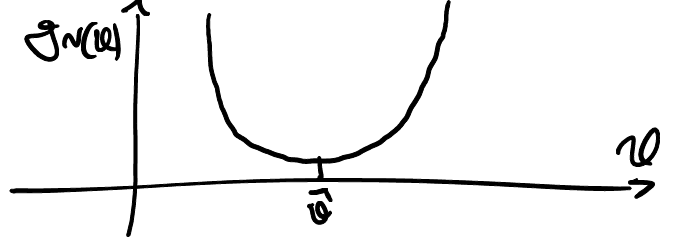
\includegraphics[width=.4\linewidth]{quadratic.png}
\end{figure}
$J_N$ is a \textbf{quadratic} function of $\theta$ : in this case it's usually easy to find the \textbf{global minimum} explicitly.\\
\textbf{AR \& ARX} models are of this kind.
\item $J(\theta) $ is \textbf{not} a quadratic function , \textbf{no local minima}\\
\begin{figure}[H]
 \centering
  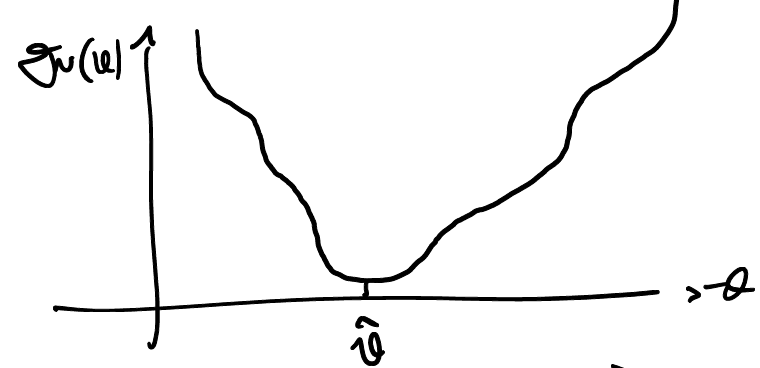
\includegraphics[width=.4\linewidth]{n_quadratic}
\end{figure}
In this case the function has no local minima so the \textbf{unique solution} is guaranteed to be found using an \textbf{iterative algorithm}.\\
\item $J(\theta)$ is \textbf{not} quadratic, \textbf{with local minima}\\
\begin{figure}[H]
 \centering
  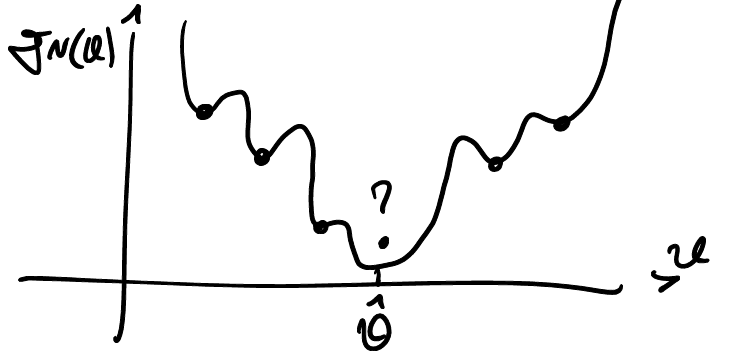
\includegraphics[width=.4\linewidth]{n_quadratic_local}
\end{figure}
In this case the function has local minima so using an \textbf{iterative algorithm} is the best way to find the unique solution which is \textbf{not guaranteed} to be found.\\
\textbf{ARMAX \& ARMA} models are of this kind.
\end{itemize}
\item \textbf{Validation}\\
The validation step checks if $m(\hat{\theta})$ can be considered a \textbf{valid} model for our purposes. Usually a technique called \textbf{cross-validation} is used.
\end{enumerate}


\subsection{Identification of ARX models}
Given an available dataset of length N :
$$ \{ u(1),u(2),...,u(N)\}$$
$$ \{ y(1),y(2),...,y(N)\}$$
An the model class \textbf{ARX(m,p+1)}:
$$ y(t) = \frac{B(Z)}{A(Z)}u(t-1)+\frac{1}{A(Z)}e(t) , e(t) \sim WN(0,\lambda^2)$$
where
 $ \theta = \begin{bmatrix}
                a_1  
                ...  
                a_m 
                b_0  
                ...  
                b_p 
             \end{bmatrix}^T$ 
is the \textbf{parameter vector} of dimension $n_{\theta} = m+p+1$.
\begin{description}
\item[Remark]\hfill\\
Using \textbf{k=1} is not a restriction but the \textbf{most general} case of an ARX. If the system has $k > 1$ we will find out during the identification process.
\end{description}
\subsubsection{Loss function: Least Squares}
The loss function for the ARX models is the \textbf{P.E.M.}:
\[
\boxed{J_N(\theta) = \frac{1}{N} \sum\limits_{t=1}^{N}(y(t)-\hat{y}(t|t-1,\theta))^2}
\]
The predictor for the model , deriving it from the  general ARMAX model, is :
$$ \hat{y}(t|t-1;\theta) = \frac{B(Z)}u(t-1)+ (1-A(Z))y(t)$$
\[
\boxed{\hat{y}(t|t-1;\theta) = b_0u(t-1)+...+b_pu(t-p-1)-a_1y(t-1)-...-a_my(t-m)}
\]

where we can define the \textbf{data vector}:
$$ \phi = \begin{bmatrix}
                -y(t-1),  
                ...  
                -y(t-m) ,
                
                u(t-1),
                ...  
                u(t-p-1) 
             \end{bmatrix}^T$$ 

so $\hat{y}(t|t-1) = \phi(t)^T \theta$ , a linear function of $\theta$. Substituting in the loss function:
$$ J_N(\theta)= \frac{1}{N} \sum\limits_{t=1}^{N}(y(t) - \phi(t)\theta)^2$$
A \textbf{quadratic} function is obtained so the \textbf{unique solution} can be found explicitly using a minimization method.To find the minimum we differentiate wrt to the parameter vector $\theta$ : 
$$ \frac{\partial{J_N(\theta)}}{\partial \theta} = 0$$
$$ \frac{\partial{J_N(\theta)}}{\partial \theta} = \frac{2}{N}\sum\limits_{t=1}^{N}\phi(t)(y(t)-\phi(t)^T\theta)$$

$$ (\sum\limits_{t=1}^{N} \phi(t)\phi(t)^T)\theta = \sum\limits_{t=1}^{N} y(t) \phi
(t)$$
Assuming that the $n_{\theta} $ x $ n_{\theta} $ matrix $\sum\limits_{t=1}^{N}\phi(t)\phi(t)^T$ matrix is \textbf{non singular } and thus \textbf{invertible}:
\[
\boxed{\hat{\theta}_N= (\sum\limits_{t=1}^{N}\phi(t)\phi(t)^T)^{-1}(\sum\limits_{t=1}^{N}y(t)\phi(t))}
\] 
This is the \textbf{explicit} solution of the ARX identification problem also known as \textbf{Least Squares}

\subsubsection{Example}
Consider a dataset of length N=10 and 
$$ y(t) = \frac{b}{1+aZ^{-1}}u(t-1)+\frac{1}{1+aZ^{-1}}e(t), e(t) \sim WN(0,\lambda^2)$$
an ARX(1,1) general model class.
Assuming that the process is in canonical representation ( $|a|<1$ must hold).
The predictor of the model is :
$$ \hat{y}(t|t-1)= \frac{B(Z)}{1}u(t-1)+\frac{1-A(Z)}{1}e(t)$$
\[
\boxed{\hat{y}(t|t-1)=bu(t-1)-ay(t-1)}
\]
and $\theta= [a,b]^T$.\\
The loss function is :
$$ J_{10}(\theta) = \frac{1}{10}\sum\limits_{t=1}^{10}(y(t) - bu(t-1)+ay(t-1))^2$$
\begin{description}
\item[Remark]\hfill\\
Since we don't have data points for t=0 , starting at time t=1 doesn't allow us to compute $-bu(0)+ay(0)$ so a modified version of the performance index is used:
\[
\boxed{J_N(\theta)= \frac{1}{N-h}\sum\limits_{t=h+1}^{N}(y(t)-\hat{y}(t|t-1))^2}
\]
where $h=max\{m,p+1\}$
\end{description}
In our case $h=max(1,1)=1$ so 
$$ J_{10}(\theta) = \frac{1}{9}\sum\limits_{t=2}^{10}(y(t) - bu(t-1)+ay(t-1))^2$$